% =====================================================================
% main.tex - two-column paper template (LaTeX + Python)
% This is the ONLY LaTeX file in the project root: build this one.
% Everything else lives in latex/ (header, bibliography, chapters,
% figures, generated/ = written by Python).
%
% TWO INDEPENDENT SWITCHES:
%   Layout:  \widetrue   -> title AND abstract span the full width
%            \widefalse  -> abstract in the first column only
%   Fonts:   \timestrue  -> Times for text, maths AND plots (mathptmx)
%            \timesfalse -> Computer Modern for text, maths AND plots
% (python/latexio.py reads the \timestrue/\timesfalse line, so the plots
%  always match the paper fonts)
% =====================================================================
\documentclass[10pt,twocolumn]{article}

\newif\ifwide
\newif\iftimes
\widetrue          % <-- layout:  \widetrue (layout 2)  or  \widefalse (layout 1)
\timesfalse         % <-- fonts:   \timestrue (Times)    or  \timesfalse (Computer Modern)

% Packages and custom commands. Use \input, not \include:
% \include is only allowed after \begin{document}.
% =====================================================================
% HEADER — pacchetti e comandi personalizzati
% Riorganizzato per chiarezza ed efficienza di compilazione.
% Sezioni:
%   1. Codifica e layout di pagina
%   2. Pacchetti matematici (AMS)
%   3. Pacchetti attivamente usati nei capitoli
%   4. Hyperref (va caricato quasi per ultimo)
%   5. Bibliografia (biblatex + biber)
%   6. Comandi personalizzati attivi
%   7. NON UTILIZZATI nella compilazione attuale (non cancellati)
%
% Righe marcate [ADDED] = aggiunte per il layout a due colonne.
% NB: questo file contiene \usepackage, quindi va caricato nel
% preambolo con % =====================================================================
% HEADER — pacchetti e comandi personalizzati
% Riorganizzato per chiarezza ed efficienza di compilazione.
% Sezioni:
%   1. Codifica e layout di pagina
%   2. Pacchetti matematici (AMS)
%   3. Pacchetti attivamente usati nei capitoli
%   4. Hyperref (va caricato quasi per ultimo)
%   5. Bibliografia (biblatex + biber)
%   6. Comandi personalizzati attivi
%   7. NON UTILIZZATI nella compilazione attuale (non cancellati)
%
% Righe marcate [ADDED] = aggiunte per il layout a due colonne.
% NB: questo file contiene \usepackage, quindi va caricato nel
% preambolo con % =====================================================================
% HEADER — pacchetti e comandi personalizzati
% Riorganizzato per chiarezza ed efficienza di compilazione.
% Sezioni:
%   1. Codifica e layout di pagina
%   2. Pacchetti matematici (AMS)
%   3. Pacchetti attivamente usati nei capitoli
%   4. Hyperref (va caricato quasi per ultimo)
%   5. Bibliografia (biblatex + biber)
%   6. Comandi personalizzati attivi
%   7. NON UTILIZZATI nella compilazione attuale (non cancellati)
%
% Righe marcate [ADDED] = aggiunte per il layout a due colonne.
% NB: questo file contiene \usepackage, quindi va caricato nel
% preambolo con \input{latex/header}, NON con \include{...}.
% =====================================================================


% ---------------------------------------------------------------
% 1. CODIFICA E LAYOUT DI PAGINA
% ---------------------------------------------------------------
\usepackage[utf8]{inputenc}
\usepackage[T1]{fontenc}
\usepackage[
    a4paper,
    left=1.9cm,                 % If you change margins/column spacing in
    right=1.9cm,                % header.tex update the two width constants
    top=2.0cm,                  % at the top of `python/latexio.py`.
    bottom=2.0cm,
    columnsep=0.7cm             % [ADDED] distanza tra le colonne
]{geometry}

% [ADDED] Font Times (testo + matematica), indipendente dal layout.
% Il flag \iftimes e' definito in main.tex (\timestrue / \timesfalse).
\iftimes
    \usepackage{mathptmx}
\fi


% ---------------------------------------------------------------
% 2. PACCHETTI MATEMATICI (AMS)
% ---------------------------------------------------------------
% Usati ovunque: \mathbb, \mathcal, align, aligned, \boldsymbol, ecc.
\usepackage{amsmath}
\usepackage{amssymb}

% ---------------------------------------------------------------
% 3. PACCHETTI ATTIVAMENTE USATI NEI CAPITOLI
% ---------------------------------------------------------------
\usepackage{cancel}       % \cancel, \bcancel, \xcancel (usati in ch1 e ch2)

\usepackage{comment}      % BUGFIX: mancava. Senza questo pacchetto gli
                          % ambienti \begin{comment}...\end{comment} in
                          % AxionEMLagrangian.tex non vengono riconosciuti:
                              % LaTeX genera errori e IL TESTO VIENE COMUNQUE
                          % STAMPATO nel PDF invece di essere nascosto.

\usepackage{booktabs}     % [ADDED] tabelle generate da Python (\toprule, \midrule, \bottomrule)

\usepackage{authblk}      % [ADDED] autori + affiliazioni (\author[1]{..}, \affil[1]{..})

% [ADDED] Apici delle affiliazioni automatici.
% Gli apici 1,2,... servono solo a dire "quale autore appartiene a quale
% affiliazione". Hanno senso SOLO se ci sono almeno 2 autori E almeno 2
% affiliazioni. In tutti gli altri casi vengono tolti:
%   1 autore,  1 affiliazione  -> nessun apice
%   1 autore,  2+ affiliazioni -> nessun apice (le affiliazioni sono tutte sue)
%   2+ autori, 1 affiliazione  -> nessun apice (sono tutti li')
%   2+ autori, 2+ affiliazioni -> apici
% Si scrive come prima: \author[1]{..} \affil[1]{..}. Le etichette
% vengono ignorate quando non servono.
\makeatletter
\newcount\autoNauth \newcount\autoNaff
% authblk definisce \author e \affil con \newcommand[2][]: \let della macro
% darebbe un "trampolino" che richiama il nome \author (cioe' questa
% stessa ridefinizione). Si salvano quindi le macro interne (forma \macro[#1]{#2}).
\expandafter\let\expandafter\autoInnerAuthor\csname\string\author\endcsname
\expandafter\let\expandafter\autoInnerAffil\csname\string\affil\endcsname
\def\autoMarked{}\def\autoPlain{}
\renewcommand{\author}[2][]{%
  \global\advance\autoNauth\@ne
  \g@addto@macro\autoMarked{\autoInnerAuthor[#1]{#2}}%
  \g@addto@macro\autoPlain{\autoInnerAuthor[]{#2}}}
\renewcommand{\affil}[2][]{%
  \global\advance\autoNaff\@ne
  \g@addto@macro\autoMarked{\autoInnerAffil[#1]{#2}}%
  \g@addto@macro\autoPlain{\autoInnerAffil[]{#2}}}
\AtBeginDocument{%
  \ifnum\autoNauth>\@ne
    \ifnum\autoNaff>\@ne \autoMarked\else\autoPlain\fi
  \else\autoPlain\fi}
\makeatother

\usepackage{xcolor}
    \definecolor{d-blue}{HTML}{000022}   % usato in hyperref (link/cite color)
    \definecolor{d-red}{HTML}{550000}
    \definecolor{d-green}{HTML}{005500}
    \definecolor{grey}{HTML}{888888}

\usepackage[
    colorlinks=true,
    linkcolor=d-blue,
    urlcolor=d-blue,
    citecolor=d-blue
]{hyperref}

\makeatletter
\renewcommand{\l@section}{\@dottedtocline{1}{1.0em}{1.8em}}
\renewcommand{\l@subsection}{\@dottedtocline{2}{2.8em}{2.6em}}
\renewcommand{\l@subsubsection}{\@dottedtocline{3}{5.4em}{3.4em}}
\makeatother
%\setlength{\parskip}{0pt}   % solo dentro il sommario, vedi sotto

\usepackage{lipsum}




% ---------------------------------------------------------------
% 4. BIBLIOGRAFIA (biblatex + biber)
% ---------------------------------------------------------------
\usepackage{csquotes}     % raccomandato da biblatex per le citazioni testuali
\usepackage[
    backend=biber,
    style=phys,          % stile APS-like per la fisica
    sorting=none,        % ordine controllato da 'sortkey' nel .bib
    biblabel=brackets,   % etichette [1], [2]... invece degli apici
    doi=true,            % IMPORTANTE: 'phys' disattiva i DOI di default
    url=true,
    eprint=false,
    giveninits=true,     % iniziali puntate: S. M. Carroll
    maxbibnames=10
]{biblatex}

% --- Layout "manuale" delle referenze -------------------------------
% Titoli in corsivo, con le maiuscole originali del .bib
% ('phys' forza il sentence case: "Planck" diventerebbe "planck")
\DeclareFieldFormat{titlecase}{#1}
\DeclareFieldFormat{title}{\emph{#1}}
\DeclareFieldFormat[article,inproceedings,patent]{title}{\emph{#1}}
\DeclareFieldFormat[book,thesis,online]{title}{\emph{#1}}

% DOI/URL stampati per esteso e cliccabili, su una riga a parte
\DeclareFieldFormat{doi}{\url{https://doi.org/#1}}
\DeclareFieldFormat{url}{\url{#1}}

\renewbibmacro*{doi+eprint+url}{%
    \iffieldundef{doi}
        {\iffieldundef{url}
            {}
            {\setunit{\addcomma\space}\printfield{url}}}
        {\setunit{\addcomma\space}\printfield{doi}}%
}
\renewbibmacro*{url+urldate}{%
    \iffieldundef{url}
        {}
        {\setunit{\addcomma\space}\printfield{url}}%
}

% Punto finale solo se la voce non termina gia con un link
\renewcommand*{\finentrypunct}{%
    \iffieldundef{doi}{\iffieldundef{url}{\addperiod}{}}{}%
}

% Evita che gli URL vengano "stirati" (https : / / www . ...)
\appto\biburlsetup{\Urlmuskip=0mu\relax}

% Preferisce il DOI all'URL quando entrambi sono presenti
\DeclareSourcemap{
  \maps[datatype=bibtex]{
    \map{
      \step[fieldsource=doi, final]
      \step[fieldset=url, null]
    }
  }
}


% ---------------------------------------------------------------
% 5. COMANDI PERSONALIZZATI ATTIVI
% ---------------------------------------------------------------

% Layout and modification
\newcommand{\ToDo}[1]{{\color{grey} \\ \noindent [To do:  #1]\\ \noindent}}   % per segnalare dove modificare
\newcommand{\?}{{\color{red}[??]}}   % per segnare dove andrà inserita una reference
\newcommand{\pRef}[1]{{\color{d-green} \detokenize{#1}}}   % per segnare dove andrà meglio citata una reference
\newcommand{\mmmhh}[1]{{\color{magenta} #1}}



%short hand for Lagrangian notation
\newcommand{\Lag}{\mathcal{L}}   % per simbolo di lagrangiana
\newcommand{\LagEM}{\mathcal{L}_{\scriptscriptstyle \mathrm{EM}}}   % per simbolo canonical kinetic term
\newcommand{\LagCFJ}{\mathcal{L}_{\scriptscriptstyle \mathrm{CFJ}}}   % per simbolo CS term in CFJ
\newcommand{\LagN}{\mathcal{L}_{\scriptscriptstyle \mathrm{N}}}   % per simbolo CS term in Ni lagrangian
\newcommand{\LagChi}{\mathcal{L}_{\raisebox{0.2ex}{\tiny$\chi$}}}   % per simbolo CS term in \chi lagrangian
\newcommand{\LagK}{\mathcal{L}_{\scriptscriptstyle \mathrm{K}}}   % per simbolo canonical kinetic term

%short hand for notation
\newcommand{\0}{,\mathrm{o}}
\newcommand{\fg}{{\scriptscriptstyle \mathrm{FG}}}
\newcommand{\cmb}{{\scriptscriptstyle \mathrm{CMB}}}
\newcommand{\TT}{{\scriptscriptstyle \mathrm{TT}}}
\newcommand{\TE}{{\scriptscriptstyle \mathrm{TE}}}
\newcommand{\TB}{{\scriptscriptstyle \mathrm{TB}}}
\newcommand{\EE}{{\scriptscriptstyle \mathrm{EE}}}
\newcommand{\BB}{{\scriptscriptstyle \mathrm{BB}}}
\newcommand{\EB}{{\scriptscriptstyle \mathrm{EB}}}




\setlength{\parskip}{3pt} % per piccole spaziature tra paragrafi

% =====================================================================
% 6. NON UTILIZZATI NELLA COMPILAZIONE ATTUALE
%    (non cancellati: tenuti pronti per quando estenderai il testo)
% =====================================================================
\usepackage{graphicx}     % \includegraphics — non ancora usato, utile
                          % appena inserirai figure/immagini.
\graphicspath{{latex/generated/}{latex/figures/}}  % [ADDED] dove cercare le figure
%\usepackage{bm}  % rimosso: non usato nel testo           % simboli in grassetto (\bm{...}) — non ancora
                          % usato (per vettori si usa \mathbf/\boldsymbol).
%\usepackage{siunitx}  % rimosso: non usato nel testo      % gestione delle unità di misura (\si, \SI, \num)
                          % — non ancora usato nel testo.
                          % ATTENZIONE: siunitx e physics possono entrare
                          % in conflitto su alcuni comandi (es. \qty):
                          % se in futuro userai entrambi, carica siunitx
                          % PRIMA di physics oppure usa le opzioni di
                          % compatibilità di physics.

% Colore definito ma non richiamato in nessun comando/testo:
% \definecolor{l-blue}{HTML}{4444FF}

% Sfondo/testo colorato — riga opzionale, disattiva la pagina bianca:
%\pagecolor[rgb]{0,0,0} %cambiare colore allo sfondo. Commentare per avere pag bianca
%\color[rgb]{0.8,0.8,0.8} %cambiare colore al testo. Commentare per avere testo nero
, NON con \include{...}.
% =====================================================================


% ---------------------------------------------------------------
% 1. CODIFICA E LAYOUT DI PAGINA
% ---------------------------------------------------------------
\usepackage[utf8]{inputenc}
\usepackage[T1]{fontenc}
\usepackage[
    a4paper,
    left=1.9cm,                 % If you change margins/column spacing in
    right=1.9cm,                % header.tex update the two width constants
    top=2.0cm,                  % at the top of `python/latexio.py`.
    bottom=2.0cm,
    columnsep=0.7cm             % [ADDED] distanza tra le colonne
]{geometry}

% [ADDED] Font Times (testo + matematica), indipendente dal layout.
% Il flag \iftimes e' definito in main.tex (\timestrue / \timesfalse).
\iftimes
    \usepackage{mathptmx}
\fi


% ---------------------------------------------------------------
% 2. PACCHETTI MATEMATICI (AMS)
% ---------------------------------------------------------------
% Usati ovunque: \mathbb, \mathcal, align, aligned, \boldsymbol, ecc.
\usepackage{amsmath}
\usepackage{amssymb}

% ---------------------------------------------------------------
% 3. PACCHETTI ATTIVAMENTE USATI NEI CAPITOLI
% ---------------------------------------------------------------
\usepackage{cancel}       % \cancel, \bcancel, \xcancel (usati in ch1 e ch2)

\usepackage{comment}      % BUGFIX: mancava. Senza questo pacchetto gli
                          % ambienti \begin{comment}...\end{comment} in
                          % AxionEMLagrangian.tex non vengono riconosciuti:
                              % LaTeX genera errori e IL TESTO VIENE COMUNQUE
                          % STAMPATO nel PDF invece di essere nascosto.

\usepackage{booktabs}     % [ADDED] tabelle generate da Python (\toprule, \midrule, \bottomrule)

\usepackage{authblk}      % [ADDED] autori + affiliazioni (\author[1]{..}, \affil[1]{..})

% [ADDED] Apici delle affiliazioni automatici.
% Gli apici 1,2,... servono solo a dire "quale autore appartiene a quale
% affiliazione". Hanno senso SOLO se ci sono almeno 2 autori E almeno 2
% affiliazioni. In tutti gli altri casi vengono tolti:
%   1 autore,  1 affiliazione  -> nessun apice
%   1 autore,  2+ affiliazioni -> nessun apice (le affiliazioni sono tutte sue)
%   2+ autori, 1 affiliazione  -> nessun apice (sono tutti li')
%   2+ autori, 2+ affiliazioni -> apici
% Si scrive come prima: \author[1]{..} \affil[1]{..}. Le etichette
% vengono ignorate quando non servono.
\makeatletter
\newcount\autoNauth \newcount\autoNaff
% authblk definisce \author e \affil con \newcommand[2][]: \let della macro
% darebbe un "trampolino" che richiama il nome \author (cioe' questa
% stessa ridefinizione). Si salvano quindi le macro interne (forma \macro[#1]{#2}).
\expandafter\let\expandafter\autoInnerAuthor\csname\string\author\endcsname
\expandafter\let\expandafter\autoInnerAffil\csname\string\affil\endcsname
\def\autoMarked{}\def\autoPlain{}
\renewcommand{\author}[2][]{%
  \global\advance\autoNauth\@ne
  \g@addto@macro\autoMarked{\autoInnerAuthor[#1]{#2}}%
  \g@addto@macro\autoPlain{\autoInnerAuthor[]{#2}}}
\renewcommand{\affil}[2][]{%
  \global\advance\autoNaff\@ne
  \g@addto@macro\autoMarked{\autoInnerAffil[#1]{#2}}%
  \g@addto@macro\autoPlain{\autoInnerAffil[]{#2}}}
\AtBeginDocument{%
  \ifnum\autoNauth>\@ne
    \ifnum\autoNaff>\@ne \autoMarked\else\autoPlain\fi
  \else\autoPlain\fi}
\makeatother

\usepackage{xcolor}
    \definecolor{d-blue}{HTML}{000022}   % usato in hyperref (link/cite color)
    \definecolor{d-red}{HTML}{550000}
    \definecolor{d-green}{HTML}{005500}
    \definecolor{grey}{HTML}{888888}

\usepackage[
    colorlinks=true,
    linkcolor=d-blue,
    urlcolor=d-blue,
    citecolor=d-blue
]{hyperref}

\makeatletter
\renewcommand{\l@section}{\@dottedtocline{1}{1.0em}{1.8em}}
\renewcommand{\l@subsection}{\@dottedtocline{2}{2.8em}{2.6em}}
\renewcommand{\l@subsubsection}{\@dottedtocline{3}{5.4em}{3.4em}}
\makeatother
%\setlength{\parskip}{0pt}   % solo dentro il sommario, vedi sotto

\usepackage{lipsum}




% ---------------------------------------------------------------
% 4. BIBLIOGRAFIA (biblatex + biber)
% ---------------------------------------------------------------
\usepackage{csquotes}     % raccomandato da biblatex per le citazioni testuali
\usepackage[
    backend=biber,
    style=phys,          % stile APS-like per la fisica
    sorting=none,        % ordine controllato da 'sortkey' nel .bib
    biblabel=brackets,   % etichette [1], [2]... invece degli apici
    doi=true,            % IMPORTANTE: 'phys' disattiva i DOI di default
    url=true,
    eprint=false,
    giveninits=true,     % iniziali puntate: S. M. Carroll
    maxbibnames=10
]{biblatex}

% --- Layout "manuale" delle referenze -------------------------------
% Titoli in corsivo, con le maiuscole originali del .bib
% ('phys' forza il sentence case: "Planck" diventerebbe "planck")
\DeclareFieldFormat{titlecase}{#1}
\DeclareFieldFormat{title}{\emph{#1}}
\DeclareFieldFormat[article,inproceedings,patent]{title}{\emph{#1}}
\DeclareFieldFormat[book,thesis,online]{title}{\emph{#1}}

% DOI/URL stampati per esteso e cliccabili, su una riga a parte
\DeclareFieldFormat{doi}{\url{https://doi.org/#1}}
\DeclareFieldFormat{url}{\url{#1}}

\renewbibmacro*{doi+eprint+url}{%
    \iffieldundef{doi}
        {\iffieldundef{url}
            {}
            {\setunit{\addcomma\space}\printfield{url}}}
        {\setunit{\addcomma\space}\printfield{doi}}%
}
\renewbibmacro*{url+urldate}{%
    \iffieldundef{url}
        {}
        {\setunit{\addcomma\space}\printfield{url}}%
}

% Punto finale solo se la voce non termina gia con un link
\renewcommand*{\finentrypunct}{%
    \iffieldundef{doi}{\iffieldundef{url}{\addperiod}{}}{}%
}

% Evita che gli URL vengano "stirati" (https : / / www . ...)
\appto\biburlsetup{\Urlmuskip=0mu\relax}

% Preferisce il DOI all'URL quando entrambi sono presenti
\DeclareSourcemap{
  \maps[datatype=bibtex]{
    \map{
      \step[fieldsource=doi, final]
      \step[fieldset=url, null]
    }
  }
}


% ---------------------------------------------------------------
% 5. COMANDI PERSONALIZZATI ATTIVI
% ---------------------------------------------------------------

% Layout and modification
\newcommand{\ToDo}[1]{{\color{grey} \\ \noindent [To do:  #1]\\ \noindent}}   % per segnalare dove modificare
\newcommand{\?}{{\color{red}[??]}}   % per segnare dove andrà inserita una reference
\newcommand{\pRef}[1]{{\color{d-green} \detokenize{#1}}}   % per segnare dove andrà meglio citata una reference
\newcommand{\mmmhh}[1]{{\color{magenta} #1}}



%short hand for Lagrangian notation
\newcommand{\Lag}{\mathcal{L}}   % per simbolo di lagrangiana
\newcommand{\LagEM}{\mathcal{L}_{\scriptscriptstyle \mathrm{EM}}}   % per simbolo canonical kinetic term
\newcommand{\LagCFJ}{\mathcal{L}_{\scriptscriptstyle \mathrm{CFJ}}}   % per simbolo CS term in CFJ
\newcommand{\LagN}{\mathcal{L}_{\scriptscriptstyle \mathrm{N}}}   % per simbolo CS term in Ni lagrangian
\newcommand{\LagChi}{\mathcal{L}_{\raisebox{0.2ex}{\tiny$\chi$}}}   % per simbolo CS term in \chi lagrangian
\newcommand{\LagK}{\mathcal{L}_{\scriptscriptstyle \mathrm{K}}}   % per simbolo canonical kinetic term

%short hand for notation
\newcommand{\0}{,\mathrm{o}}
\newcommand{\fg}{{\scriptscriptstyle \mathrm{FG}}}
\newcommand{\cmb}{{\scriptscriptstyle \mathrm{CMB}}}
\newcommand{\TT}{{\scriptscriptstyle \mathrm{TT}}}
\newcommand{\TE}{{\scriptscriptstyle \mathrm{TE}}}
\newcommand{\TB}{{\scriptscriptstyle \mathrm{TB}}}
\newcommand{\EE}{{\scriptscriptstyle \mathrm{EE}}}
\newcommand{\BB}{{\scriptscriptstyle \mathrm{BB}}}
\newcommand{\EB}{{\scriptscriptstyle \mathrm{EB}}}




\setlength{\parskip}{3pt} % per piccole spaziature tra paragrafi

% =====================================================================
% 6. NON UTILIZZATI NELLA COMPILAZIONE ATTUALE
%    (non cancellati: tenuti pronti per quando estenderai il testo)
% =====================================================================
\usepackage{graphicx}     % \includegraphics — non ancora usato, utile
                          % appena inserirai figure/immagini.
\graphicspath{{latex/generated/}{latex/figures/}}  % [ADDED] dove cercare le figure
%\usepackage{bm}  % rimosso: non usato nel testo           % simboli in grassetto (\bm{...}) — non ancora
                          % usato (per vettori si usa \mathbf/\boldsymbol).
%\usepackage{siunitx}  % rimosso: non usato nel testo      % gestione delle unità di misura (\si, \SI, \num)
                          % — non ancora usato nel testo.
                          % ATTENZIONE: siunitx e physics possono entrare
                          % in conflitto su alcuni comandi (es. \qty):
                          % se in futuro userai entrambi, carica siunitx
                          % PRIMA di physics oppure usa le opzioni di
                          % compatibilità di physics.

% Colore definito ma non richiamato in nessun comando/testo:
% \definecolor{l-blue}{HTML}{4444FF}

% Sfondo/testo colorato — riga opzionale, disattiva la pagina bianca:
%\pagecolor[rgb]{0,0,0} %cambiare colore allo sfondo. Commentare per avere pag bianca
%\color[rgb]{0.8,0.8,0.8} %cambiare colore al testo. Commentare per avere testo nero
, NON con \include{...}.
% =====================================================================


% ---------------------------------------------------------------
% 1. CODIFICA E LAYOUT DI PAGINA
% ---------------------------------------------------------------
\usepackage[utf8]{inputenc}
\usepackage[T1]{fontenc}
\usepackage[
    a4paper,
    left=1.9cm,                 % If you change margins/column spacing in
    right=1.9cm,                % header.tex update the two width constants
    top=2.0cm,                  % at the top of `python/latexio.py`.
    bottom=2.0cm,
    columnsep=0.7cm             % [ADDED] distanza tra le colonne
]{geometry}

% [ADDED] Font Times (testo + matematica), indipendente dal layout.
% Il flag \iftimes e' definito in main.tex (\timestrue / \timesfalse).
\iftimes
    \usepackage{mathptmx}
\fi


% ---------------------------------------------------------------
% 2. PACCHETTI MATEMATICI (AMS)
% ---------------------------------------------------------------
% Usati ovunque: \mathbb, \mathcal, align, aligned, \boldsymbol, ecc.
\usepackage{amsmath}
\usepackage{amssymb}

% ---------------------------------------------------------------
% 3. PACCHETTI ATTIVAMENTE USATI NEI CAPITOLI
% ---------------------------------------------------------------
\usepackage{cancel}       % \cancel, \bcancel, \xcancel (usati in ch1 e ch2)

\usepackage{comment}      % BUGFIX: mancava. Senza questo pacchetto gli
                          % ambienti \begin{comment}...\end{comment} in
                          % AxionEMLagrangian.tex non vengono riconosciuti:
                              % LaTeX genera errori e IL TESTO VIENE COMUNQUE
                          % STAMPATO nel PDF invece di essere nascosto.

\usepackage{booktabs}     % [ADDED] tabelle generate da Python (\toprule, \midrule, \bottomrule)

\usepackage{authblk}      % [ADDED] autori + affiliazioni (\author[1]{..}, \affil[1]{..})

% [ADDED] Apici delle affiliazioni automatici.
% Gli apici 1,2,... servono solo a dire "quale autore appartiene a quale
% affiliazione". Hanno senso SOLO se ci sono almeno 2 autori E almeno 2
% affiliazioni. In tutti gli altri casi vengono tolti:
%   1 autore,  1 affiliazione  -> nessun apice
%   1 autore,  2+ affiliazioni -> nessun apice (le affiliazioni sono tutte sue)
%   2+ autori, 1 affiliazione  -> nessun apice (sono tutti li')
%   2+ autori, 2+ affiliazioni -> apici
% Si scrive come prima: \author[1]{..} \affil[1]{..}. Le etichette
% vengono ignorate quando non servono.
\makeatletter
\newcount\autoNauth \newcount\autoNaff
% authblk definisce \author e \affil con \newcommand[2][]: \let della macro
% darebbe un "trampolino" che richiama il nome \author (cioe' questa
% stessa ridefinizione). Si salvano quindi le macro interne (forma \macro[#1]{#2}).
\expandafter\let\expandafter\autoInnerAuthor\csname\string\author\endcsname
\expandafter\let\expandafter\autoInnerAffil\csname\string\affil\endcsname
\def\autoMarked{}\def\autoPlain{}
\renewcommand{\author}[2][]{%
  \global\advance\autoNauth\@ne
  \g@addto@macro\autoMarked{\autoInnerAuthor[#1]{#2}}%
  \g@addto@macro\autoPlain{\autoInnerAuthor[]{#2}}}
\renewcommand{\affil}[2][]{%
  \global\advance\autoNaff\@ne
  \g@addto@macro\autoMarked{\autoInnerAffil[#1]{#2}}%
  \g@addto@macro\autoPlain{\autoInnerAffil[]{#2}}}
\AtBeginDocument{%
  \ifnum\autoNauth>\@ne
    \ifnum\autoNaff>\@ne \autoMarked\else\autoPlain\fi
  \else\autoPlain\fi}
\makeatother

\usepackage{xcolor}
    \definecolor{d-blue}{HTML}{000022}   % usato in hyperref (link/cite color)
    \definecolor{d-red}{HTML}{550000}
    \definecolor{d-green}{HTML}{005500}
    \definecolor{grey}{HTML}{888888}

\usepackage[
    colorlinks=true,
    linkcolor=d-blue,
    urlcolor=d-blue,
    citecolor=d-blue
]{hyperref}

\makeatletter
\renewcommand{\l@section}{\@dottedtocline{1}{1.0em}{1.8em}}
\renewcommand{\l@subsection}{\@dottedtocline{2}{2.8em}{2.6em}}
\renewcommand{\l@subsubsection}{\@dottedtocline{3}{5.4em}{3.4em}}
\makeatother
%\setlength{\parskip}{0pt}   % solo dentro il sommario, vedi sotto

\usepackage{lipsum}




% ---------------------------------------------------------------
% 4. BIBLIOGRAFIA (biblatex + biber)
% ---------------------------------------------------------------
\usepackage{csquotes}     % raccomandato da biblatex per le citazioni testuali
\usepackage[
    backend=biber,
    style=phys,          % stile APS-like per la fisica
    sorting=none,        % ordine controllato da 'sortkey' nel .bib
    biblabel=brackets,   % etichette [1], [2]... invece degli apici
    doi=true,            % IMPORTANTE: 'phys' disattiva i DOI di default
    url=true,
    eprint=false,
    giveninits=true,     % iniziali puntate: S. M. Carroll
    maxbibnames=10
]{biblatex}

% --- Layout "manuale" delle referenze -------------------------------
% Titoli in corsivo, con le maiuscole originali del .bib
% ('phys' forza il sentence case: "Planck" diventerebbe "planck")
\DeclareFieldFormat{titlecase}{#1}
\DeclareFieldFormat{title}{\emph{#1}}
\DeclareFieldFormat[article,inproceedings,patent]{title}{\emph{#1}}
\DeclareFieldFormat[book,thesis,online]{title}{\emph{#1}}

% DOI/URL stampati per esteso e cliccabili, su una riga a parte
\DeclareFieldFormat{doi}{\url{https://doi.org/#1}}
\DeclareFieldFormat{url}{\url{#1}}

\renewbibmacro*{doi+eprint+url}{%
    \iffieldundef{doi}
        {\iffieldundef{url}
            {}
            {\setunit{\addcomma\space}\printfield{url}}}
        {\setunit{\addcomma\space}\printfield{doi}}%
}
\renewbibmacro*{url+urldate}{%
    \iffieldundef{url}
        {}
        {\setunit{\addcomma\space}\printfield{url}}%
}

% Punto finale solo se la voce non termina gia con un link
\renewcommand*{\finentrypunct}{%
    \iffieldundef{doi}{\iffieldundef{url}{\addperiod}{}}{}%
}

% Evita che gli URL vengano "stirati" (https : / / www . ...)
\appto\biburlsetup{\Urlmuskip=0mu\relax}

% Preferisce il DOI all'URL quando entrambi sono presenti
\DeclareSourcemap{
  \maps[datatype=bibtex]{
    \map{
      \step[fieldsource=doi, final]
      \step[fieldset=url, null]
    }
  }
}


% ---------------------------------------------------------------
% 5. COMANDI PERSONALIZZATI ATTIVI
% ---------------------------------------------------------------

% Layout and modification
\newcommand{\ToDo}[1]{{\color{grey} \\ \noindent [To do:  #1]\\ \noindent}}   % per segnalare dove modificare
\newcommand{\?}{{\color{red}[??]}}   % per segnare dove andrà inserita una reference
\newcommand{\pRef}[1]{{\color{d-green} \detokenize{#1}}}   % per segnare dove andrà meglio citata una reference
\newcommand{\mmmhh}[1]{{\color{magenta} #1}}



%short hand for Lagrangian notation
\newcommand{\Lag}{\mathcal{L}}   % per simbolo di lagrangiana
\newcommand{\LagEM}{\mathcal{L}_{\scriptscriptstyle \mathrm{EM}}}   % per simbolo canonical kinetic term
\newcommand{\LagCFJ}{\mathcal{L}_{\scriptscriptstyle \mathrm{CFJ}}}   % per simbolo CS term in CFJ
\newcommand{\LagN}{\mathcal{L}_{\scriptscriptstyle \mathrm{N}}}   % per simbolo CS term in Ni lagrangian
\newcommand{\LagChi}{\mathcal{L}_{\raisebox{0.2ex}{\tiny$\chi$}}}   % per simbolo CS term in \chi lagrangian
\newcommand{\LagK}{\mathcal{L}_{\scriptscriptstyle \mathrm{K}}}   % per simbolo canonical kinetic term

%short hand for notation
\newcommand{\0}{,\mathrm{o}}
\newcommand{\fg}{{\scriptscriptstyle \mathrm{FG}}}
\newcommand{\cmb}{{\scriptscriptstyle \mathrm{CMB}}}
\newcommand{\TT}{{\scriptscriptstyle \mathrm{TT}}}
\newcommand{\TE}{{\scriptscriptstyle \mathrm{TE}}}
\newcommand{\TB}{{\scriptscriptstyle \mathrm{TB}}}
\newcommand{\EE}{{\scriptscriptstyle \mathrm{EE}}}
\newcommand{\BB}{{\scriptscriptstyle \mathrm{BB}}}
\newcommand{\EB}{{\scriptscriptstyle \mathrm{EB}}}




\setlength{\parskip}{3pt} % per piccole spaziature tra paragrafi

% =====================================================================
% 6. NON UTILIZZATI NELLA COMPILAZIONE ATTUALE
%    (non cancellati: tenuti pronti per quando estenderai il testo)
% =====================================================================
\usepackage{graphicx}     % \includegraphics — non ancora usato, utile
                          % appena inserirai figure/immagini.
\graphicspath{{latex/generated/}{latex/figures/}}  % [ADDED] dove cercare le figure
%\usepackage{bm}  % rimosso: non usato nel testo           % simboli in grassetto (\bm{...}) — non ancora
                          % usato (per vettori si usa \mathbf/\boldsymbol).
%\usepackage{siunitx}  % rimosso: non usato nel testo      % gestione delle unità di misura (\si, \SI, \num)
                          % — non ancora usato nel testo.
                          % ATTENZIONE: siunitx e physics possono entrare
                          % in conflitto su alcuni comandi (es. \qty):
                          % se in futuro userai entrambi, carica siunitx
                          % PRIMA di physics oppure usa le opzioni di
                          % compatibilità di physics.

% Colore definito ma non richiamato in nessun comando/testo:
% \definecolor{l-blue}{HTML}{4444FF}

% Sfondo/testo colorato — riga opzionale, disattiva la pagina bianca:
%\pagecolor[rgb]{0,0,0} %cambiare colore allo sfondo. Commentare per avere pag bianca
%\color[rgb]{0.8,0.8,0.8} %cambiare colore al testo. Commentare per avere testo nero


\addbibresource{latex/references.bib}

% Numbers computed by python/compute.py (\newcommand definitions).
% This file is created when compute.py runs, i.e. at the first build.
% AUTO-GENERATED by compute.py - do not edit by hand
\newcommand{\ellA}{\ensuremath{300}}
\newcommand{\ellD}{\ensuremath{1.20\times10^{3}}}
\newcommand{\Npeaks}{\ensuremath{6}}
\newcommand{\Hone}{\ensuremath{4.70\times10^{3}}}


% ---------------------------------------------------------------------
% Title block (superscripts appear automatically only when needed)
% ---------------------------------------------------------------------
\title{Working Title of the Paper}
\author[1]{Mirco Bridda}
%\author[2]{Second Author}
\affil[1]{Department of Physics, University of Padova, Padova, Italy}
%\affil[2]{Institute of Astronomy, University of Cambridge, Cambridge, UK}
\date{\today}

% The abstract text is defined once and used by both layouts.
\newcommand{\abstracttext}{%
  Write the abstract here. Lorem ipsum dolor sit amet, consectetur adipiscing
  elit, sed do eiusmod tempor incididunt ut labore et dolore magna aliqua.
  The polarization of the CMB is a probe of the physics of last scattering
  \cite{HW97}.%
}

\begin{document}

  \makeatletter
  \ifwide
    \twocolumn[
      \begin{@twocolumnfalse}
        \maketitle
        \begin{abstract}\abstracttext\end{abstract}
        \vspace{1.5em}
      \end{@twocolumnfalse}
    ]
  \else
    \maketitle
    \begin{abstract}\abstracttext\end{abstract}
  \fi
  \makeatother

  % ---------------------------------------------------------------------

  % Chapters/sections kept in their own files: latex/chapters/*.tex
  % (\input, not \include: \include forces a page break).
  % Example of a section kept in its own file (latex/chapters/example.tex).
% It has no \documentclass or \begin{document}: it is only pasted into main.tex.
% First line of such files, so that Ctrl+Alt+B works from this tab too:
% !TEX root = ../../main.tex
\section{Introduction}
\label{s:intro}
    Thomson scattering of a quadrupole anisotropy generates linear polarization \cite{SZ97,KKS97}.
    \lipsum[1]

  % Example of a section kept in its own file (latex/chapters/example.tex).
% It has no \documentclass or \begin{document}: it is only pasted into main.tex.
% First line of such files, so that Ctrl+Alt+B works from this tab too:
% !TEX root = ../../main.tex
\section{Results from the Python code}
    \label{s:results}
    % Numbers: write the macro defined in compute.py (here \ellA, \ellD, \Npeaks, \Hone).
    In the toy model the acoustic scale is $\ell_A=\ellA$ and the damping scale
    is $\ell_D=\ellD$. The spectrum has \Npeaks\ peaks below the multipole cut-off,
    and the first one has height $\Hone\,\mu\mathrm{K}^2$ (Table~\ref{tab:peaks}
    and Fig.~\ref{fig:spectrum}).

    % Table: latex/generated/table_peaks.tex is a bare tabular.
    \begin{table}[h]
        \centering
        \caption{First peaks of the toy spectrum (written by \texttt{compute.py}).}
        \label{tab:peaks}
        % AUTO-GENERATED by compute.py - do not edit by hand
\begin{tabular}{lcc}
\toprule
Peak & $\ell_{\rm peak}$ & Height [$\mu$K$^2$] \\
\midrule
$1$ & $298$ & $4.70\times10^{3}$ \\
$2$ & $596$ & $3.90\times10^{3}$ \\
$3$ & $894$ & $2.86\times10^{3}$ \\
$4$ & $1192$ & $1.85\times10^{3}$ \\
\bottomrule
\end{tabular}

    \end{table}

    % Plot: written by Python, exactly one column wide. \graphicspath (header.tex)
    % already points to latex/generated/ and latex/figures/, so the name is enough.
    % For a full-width plot use new_figure("full") in compute.py and a figure* here.
    \begin{figure}[t]
        \centering
        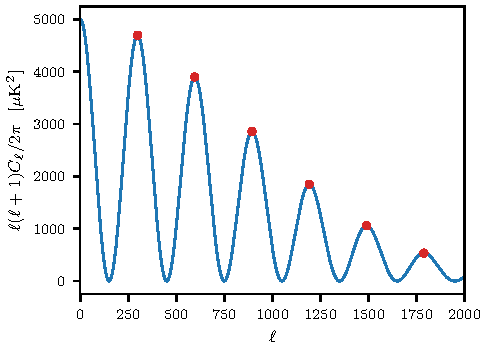
\includegraphics[width=\columnwidth]{fig_spectrum.pdf}
        \caption{Toy power spectrum (written by \texttt{compute.py}).}
        \label{fig:spectrum}
    \end{figure}

    
  % Example of a section kept in its own file (latex/chapters/example.tex).
% It has no \documentclass or \begin{document}: it is only pasted into main.tex.
% First line of such files, so that Ctrl+Alt+B works from this tab too:
% !TEX root = ../../main.tex
\section{Equations}
    \label{s:eq}
    The angular power spectra are
    \begin{equation}
        C_\ell^{XY} = 4\pi \int d\ln k\;\mathcal{P}(k)\,\Delta_{X\ell}(k)\,\Delta_{Y\ell}(k),
        \label{eq:cl}
    \end{equation}
    with $X,Y\in\{T,E,B\}$. Equation~\eqref{eq:cl} is discussed in Sec.~\ref{s:intro}.
    Your shorthand commands work as before, e.g.\ $C_\ell^{\TE}$, $C_\ell^{\EE}$, $C_\ell^{\BB}$.

    \lipsum[3]

  % Example of a section kept in its own file (latex/chapters/example.tex).
% It has no \documentclass or \begin{document}: it is only pasted into main.tex.
% First line of such files, so that Ctrl+Alt+B works from this tab too:
% !TEX root = ../../main.tex
\section{Conclusions}
    \label{s:Conclusions}
    \lipsum[4]


  % ---------------------------------------------------------------------
  % Bibliography (biblatex + biber, entries in latex/references.bib)
  % ---------------------------------------------------------------------
  \printbibliography

\end{document}
